\begin{minipage}[t]{0.49\linewidth}\centering
{\color{black}\normalsize\bfseries LLM + RAG}\par\smallskip
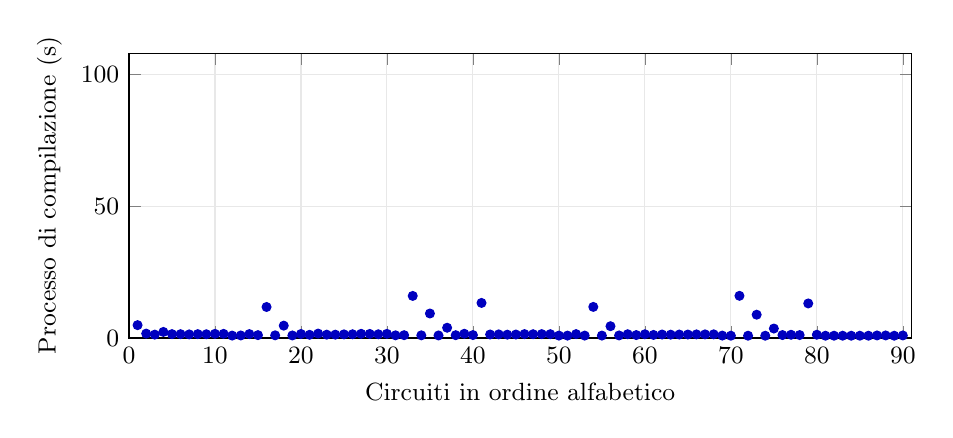
\begin{tikzpicture}\begin{axis}[width=0.95\linewidth,height=5.2cm,grid=major,grid style={gray!18},tick label style={font=\small},label style={font=\small},scaled ticks=false,/pgf/number format/use comma,unbounded coords=discard,xlabel={Circuiti in ordine alfabetico},ylabel={Processo di compilazione (s)},xmin=0,xmax=91,ymin=0,ymax=108.18607510511997,]
\addplot[color=blue!75!black,mark=*,mark size=1.6pt,only marks] coordinates {(1,4.885685760999991) (2,1.659521529000017) (3,1.2822502520000398) (4,2.3011055790000228) (5,1.4713740670000561) (6,1.4555973589999667) (7,1.3693695230000458) (8,1.4705338950000169) (9,1.4230442159999939) (10,1.5759383529999695) (11,1.574903930000005) (12,0.9162120080000022) (13,0.9664079879999008) (14,1.4864690530000644) (15,1.0889064730000655) (16,11.773682811999947) (17,1.016825995999966) (18,4.686838189000014) (19,0.9663654439999618) (20,1.5214212529999713) (21,1.2167173850000381) (22,1.6716479839999465) (23,1.2671430120001332) (24,1.267045853999889) (25,1.3798766179997983) (26,1.4241873009998471) (27,1.5872900969998227) (28,1.5419624119999753) (29,1.4174315090001528) (30,1.5741508749999866) (31,1.0167580290001297) (32,1.0698834169998008) (33,15.976622140000018) (34,1.0165207029999692) (35,9.301401043999931) (36,0.966347960000121) (37,3.8945262150000417) (38,1.0667631500000425) (39,1.607741502999943) (40,1.1179324120000729) (41,13.314986264000026) (42,1.3330600709998635) (43,1.3735714169999937) (44,1.2680016150000029) (45,1.317339015000016) (46,1.4832435990001613) (47,1.4389539670000886) (48,1.474348682000027) (49,1.452791230999992) (50,0.9173692869999286) (51,0.916983952999999) (52,1.4762099510001008) (53,0.9171883579999758) (54,11.809573294000074) (55,0.916933907999919) (56,4.479935267999963) (57,0.9667614330001015) (58,1.4292431409999153) (59,1.1171905219998735) (60,1.425462852000237) (61,1.1669257130001824) (62,1.3228949529998317) (63,1.2679540809999708) (64,1.3177758110000468) (65,1.3194896869999866) (66,1.37124201000006) (67,1.3775805679997575) (68,1.3921448769997369) (69,0.9203580309999779) (70,0.8728366079999432) (71,16.01416935799989) (72,0.8667635520000658) (73,8.843930167000053) (74,0.8668965669999125) (75,3.593396306000159) (76,1.1175996040001337) (77,1.2216010180000012) (78,1.1172829320003075) (79,13.121580164999614) (80,1.2367840110000543) (81,0.8667649099998016) (82,0.8667490230000112) (83,0.8673612440002216) (84,0.8669430509999074) (85,0.8662021029999778) (86,0.8674568289998206) (87,0.9673562320003839) (88,0.9681889080002293) (89,0.8663870360001056) (90,0.9668706590000511)};
\end{axis}\end{tikzpicture}
\end{minipage}
\hfill\begin{minipage}[t]{0.49\linewidth}\centering
{\color{black}\normalsize\bfseries LLM no RAG}\par\smallskip
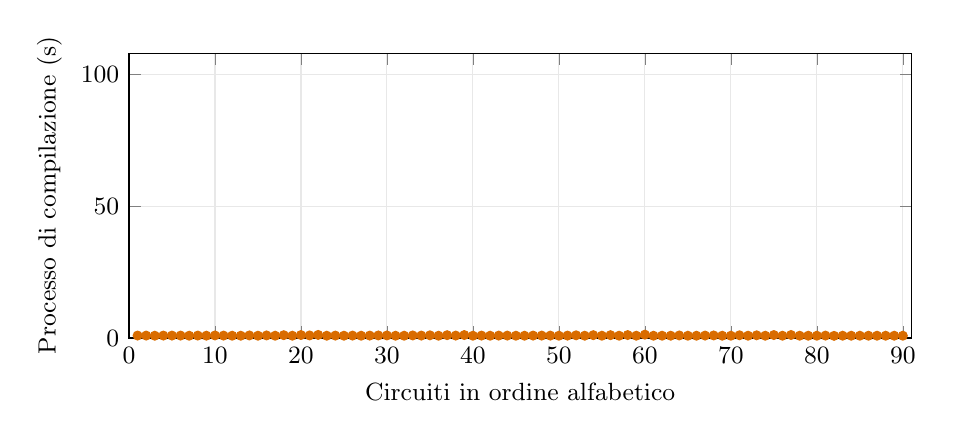
\begin{tikzpicture}\begin{axis}[width=0.95\linewidth,height=5.2cm,grid=major,grid style={gray!18},tick label style={font=\small},label style={font=\small},scaled ticks=false,/pgf/number format/use comma,unbounded coords=discard,xlabel={Circuiti in ordine alfabetico},ylabel={Processo di compilazione (s)},xmin=0,xmax=91,ymin=0,ymax=108.18607510511997,]
\addplot[color=orange!85!black,mark=*,mark size=1.6pt,only marks] coordinates {(1,0.927692386999297) (2,0.9170136559996536) (3,0.8665911170000982) (4,0.9166121540001768) (5,0.9170006969998212) (6,0.9169977760002439) (7,0.8663562080000702) (8,0.921434502000011) (9,0.8804782829993201) (10,0.9669165149998662) (11,0.916794948999268) (12,0.8667190129999653) (13,0.8662305010002456) (14,0.9674661919998471) (15,0.8668740330003857) (16,0.9694666149998739) (17,0.8671832750005706) (18,1.0692005789996983) (19,0.8669928749995961) (20,1.1201156999995874) (21,0.9680325290000837) (22,1.1711972690000039) (23,0.8669655550002062) (24,0.9167711669997516) (25,0.8667464790005397) (26,0.917037837000862) (27,0.8668490809996001) (28,0.9166725619998033) (29,0.9669696029995976) (30,0.9668746139996074) (31,0.8667161610001131) (32,0.8677475209997283) (33,0.9668413770004918) (34,0.9174060400000599) (35,1.0169887600004586) (36,0.8670428599998559) (37,1.0669406229999367) (38,0.9169508140003018) (39,1.1214497869996194) (40,0.8673651279996193) (41,0.9170616470000823) (42,0.8668370340001275) (43,0.9169078999993872) (44,0.9171750289997362) (45,0.8666465510004855) (46,0.8668612880001092) (47,0.9170519790004619) (48,0.9179833280004459) (49,0.9166967219998696) (50,0.8670053999994707) (51,0.9174349610002537) (52,1.016926581000007) (53,0.8672660799993537) (54,1.074082083000576) (55,0.867722627999683) (56,1.070627193999826) (57,0.86677426299957) (58,1.1169377680007528) (59,0.8674482389997138) (60,1.2695975640008328) (61,0.8667163479994997) (62,0.8668497080007) (63,0.8668490709997059) (64,0.967236614000285) (65,0.8662192390002019) (66,0.8684894979996898) (67,0.9182189729999664) (68,0.9667612610001015) (69,0.8664810150003177) (70,0.8664053450002029) (71,1.029937675999463) (72,0.866577580000012) (73,1.0166706469999554) (74,0.8663853990001371) (75,1.120851186999971) (76,0.866334987999835) (77,1.1393787999995766) (78,0.8664462570004616) (79,0.8678960020006343) (80,0.8672012110000651) (81,0.9170499129995733) (82,0.8159825899992939) (83,0.8663003040001058) (84,0.8670702749996053) (85,0.8667976229999113) (86,0.8666318219993627) (87,0.8675466949998736) (88,0.8666787390002355) (89,0.8668717379996451) (90,0.8664881690001494)};
\end{axis}\end{tikzpicture}
\end{minipage}
\par\vspace{0.25cm}\begin{minipage}[t]{0.49\linewidth}\centering
{\color{black}\normalsize\bfseries MQT Predictor}\par\smallskip
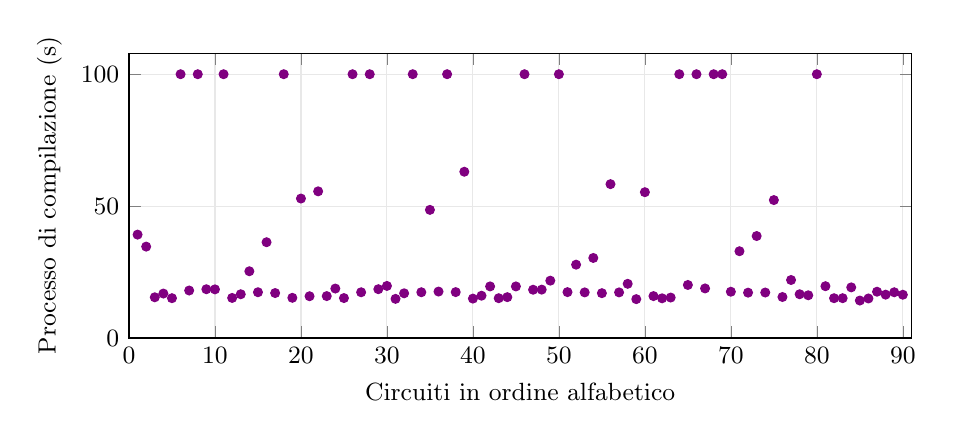
\begin{tikzpicture}\begin{axis}[width=0.95\linewidth,height=5.2cm,grid=major,grid style={gray!18},tick label style={font=\small},label style={font=\small},scaled ticks=false,/pgf/number format/use comma,unbounded coords=discard,xlabel={Circuiti in ordine alfabetico},ylabel={Processo di compilazione (s)},xmin=0,xmax=91,ymin=0,ymax=108.18607510511997,]
\addplot[color=violet,mark=*,mark size=1.6pt,only marks] coordinates {(1,39.253875307999806) (2,34.69434260299931) (3,15.458061373000419) (4,16.87410221800019) (5,15.119791938000162) (6,100.15967396300039) (7,18.027809956000056) (8,100.16216366799927) (9,18.51536186300018) (10,18.467882453999664) (11,100.16326017599931) (12,15.208549751000646) (13,16.612538584000504) (14,25.34193049300029) (15,17.374053489999824) (16,36.367063198000324) (17,17.067011914999966) (18,100.17039801600004) (19,15.25629341199965) (20,52.95246524200047) (21,15.859893324999575) (22,55.69000276400038) (23,15.911637356000028) (24,18.772898807000274) (25,15.16064676499991) (26,100.15923036999993) (27,17.36334033700041) (28,100.15821526899981) (29,18.532665263000126) (30,19.77095772099983) (31,14.860154650000368) (32,16.97285459700015) (33,100.17229176399997) (34,17.37255990199992) (35,48.64873299200008) (36,17.631611454999984) (37,100.16487753199999) (38,17.424727315999917) (39,63.13204950999989) (40,14.9569887560001) (41,16.060733840000466) (42,19.590657231000478) (43,15.1109132520005) (44,15.508460252000077) (45,19.583829274999516) (46,100.16242648799926) (47,18.325448737999977) (48,18.36881094599994) (49,21.771930343999884) (50,100.16359888500028) (51,17.421932725999795) (52,27.841695246999734) (53,17.316311329999735) (54,30.390954202000103) (55,17.020341679000012) (56,58.41948253800001) (57,17.316822931000388) (58,20.572582138999678) (59,14.757625588999872) (60,55.36427809900033) (61,15.913708068000233) (62,15.073104148999846) (63,15.359915805999663) (64,100.16358528900037) (65,20.138281515000017) (66,100.16066593600044) (67,18.818621374999566) (68,100.16040991099999) (69,100.16475099000036) (70,17.56835143799981) (71,32.951525108999704) (72,17.215895549999914) (73,38.717588493999756) (74,17.265404165999826) (75,52.371467394999854) (76,15.568297503000394) (77,22.024119859000166) (78,16.612025421999533) (79,16.219923034999738) (80,100.15999020600066) (81,19.672174512999845) (82,15.110812570000235) (83,15.117744070000299) (84,19.219604464999975) (85,14.221409050999682) (86,15.008094361000076) (87,17.57037512199986) (88,16.46072828100023) (89,17.365274191000026) (90,16.425119278999773)};
\end{axis}\end{tikzpicture}
\end{minipage}
\hfill\begin{minipage}[t]{0.49\linewidth}\centering
{\color{black}\normalsize\bfseries Random}\par\smallskip
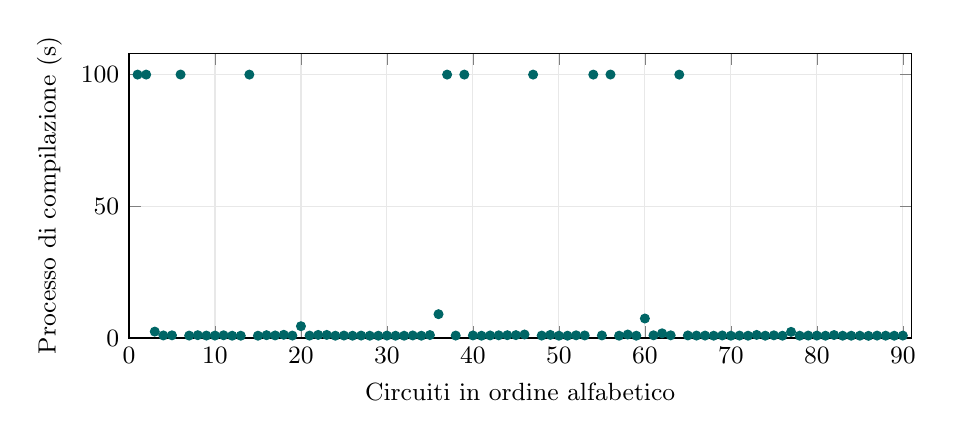
\begin{tikzpicture}\begin{axis}[width=0.95\linewidth,height=5.2cm,grid=major,grid style={gray!18},tick label style={font=\small},label style={font=\small},scaled ticks=false,/pgf/number format/use comma,unbounded coords=discard,xlabel={Circuiti in ordine alfabetico},ylabel={Processo di compilazione (s)},xmin=0,xmax=91,ymin=0,ymax=108.18607510511997,]
\addplot[color=teal!80!black,mark=*,mark size=1.6pt,only marks] coordinates {(1,100.01603336400012) (2,100.01446677800004) (3,2.4254939209999975) (4,0.9668980829997054) (5,1.0173860009999771) (6,100.03789432800022) (7,0.9169833209998615) (8,1.0674816330001704) (9,0.9174806579999313) (10,0.9166838310002277) (11,1.0297555689999172) (12,0.866801568000028) (13,0.8666439000003265) (14,100.01567727600013) (15,0.8665810659999806) (16,1.0675906070000565) (17,0.9669807959999162) (18,1.217729285999667) (19,0.9222307540003385) (20,4.478550022000036) (21,0.9167598689996339) (22,1.1671475269999974) (23,1.1673190989999966) (24,0.8666239579997637) (25,0.9344173889999183) (26,0.8668201899999985) (27,0.9261530620001395) (28,0.8691540740001074) (29,0.8662625259999004) (30,0.9172548870001265) (31,0.8664460220002184) (32,0.86641570699976) (33,0.9664724630001729) (34,0.8674182549998477) (35,1.1175419819996932) (36,9.044109287000083) (37,100.01627815500024) (38,0.9165273599996908) (39,100.01903812799992) (40,0.967749645999902) (41,0.8675621610000235) (42,0.9673360799997681) (43,1.018133347999992) (44,1.0620581439998205) (45,1.088468642999942) (46,1.3201359569998203) (47,100.01467437700012) (48,0.9177467529998466) (49,1.1718918710002981) (50,0.8671345520001523) (51,0.8732262030002858) (52,1.0198540159999538) (53,0.9665532960002565) (54,100.01423493500033) (55,0.9669041369998013) (56,100.03914649299986) (57,0.8672918769998432) (58,1.317919926000286) (59,0.8666100070004177) (60,7.402789097000095) (61,1.018922276000012) (62,1.7749337820005167) (63,1.0173219090002021) (64,100.01645778800048) (65,0.9669303380005658) (66,0.9170037650001177) (67,0.9168051190008555) (68,0.8700368419995357) (69,0.9667990859998099) (70,0.86690679000003) (71,0.9194144170005529) (72,0.8669623659998251) (73,1.1671303170005558) (74,0.8762966979993507) (75,1.0164130180000939) (76,0.8660944490002294) (77,2.32713461899948) (78,0.8680371740001647) (79,0.9228437719993963) (80,0.9165822150007443) (81,0.8668832429993927) (82,1.1174228830004722) (83,0.8671792779996395) (84,0.8667032140001538) (85,0.8667888879999737) (86,0.8166353260003234) (87,0.9168711539996366) (88,0.8833442220002325) (89,0.867958295999415) (90,0.9175392019997162)};
\end{axis}\end{tikzpicture}
\end{minipage}
\par\vspace{0.25cm}\makebox[\linewidth][c]{%
\begin{minipage}[t]{0.49\linewidth}\centering
{\color{black}\normalsize\bfseries LLM + Random RAG}\par\smallskip
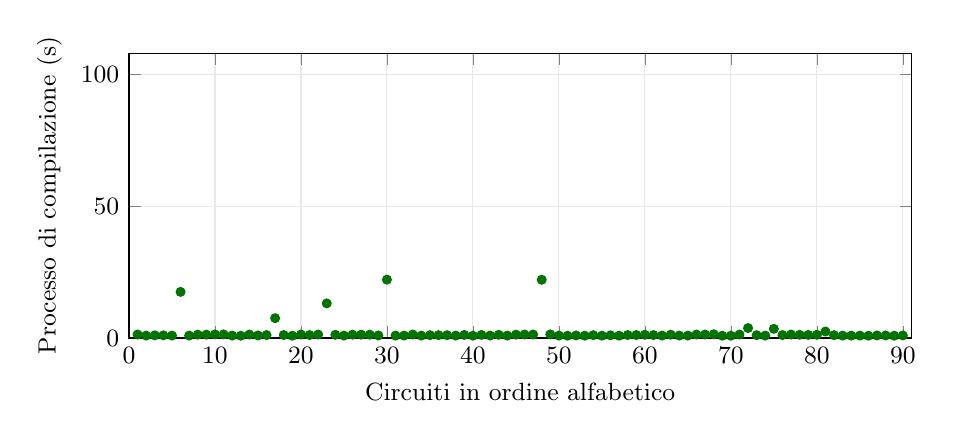
\begin{tikzpicture}\begin{axis}[width=0.95\linewidth,height=5.2cm,grid=major,grid style={gray!18},tick label style={font=\small},label style={font=\small},scaled ticks=false,/pgf/number format/use comma,unbounded coords=discard,xlabel={Circuiti in ordine alfabetico},ylabel={Processo di compilazione (s)},xmin=0,xmax=91,ymin=0,ymax=108.18607510511997,]
\addplot[color=green!45!black,mark=*,mark size=1.6pt,only marks] coordinates {(1,1.3180743670000084) (2,0.9175424809999981) (3,1.016736676999983) (4,1.0164191640000126) (5,0.9169651670000007) (6,17.505049971999995) (7,0.9167988129999571) (8,1.2674470080000901) (9,1.2675391650000165) (10,1.3683257740000272) (11,1.3677126849999013) (12,0.9173845159999701) (13,0.8662133220000214) (14,1.3189433730000246) (15,0.9671215910000228) (16,1.1193318069999805) (17,7.532046316999981) (18,1.1187757010000041) (19,0.8666086820001055) (20,1.3202210470000182) (21,1.116976789999967) (22,1.3216079669999772) (23,13.144584880000025) (24,1.2172630329999947) (25,0.9164350280000235) (26,1.2675451479999538) (27,1.2678104660001281) (28,1.2679019750000862) (29,0.9667872550000993) (30,22.163806518) (31,0.9168756400001712) (32,0.918083931999945) (33,1.3172141979998742) (34,0.9168756059998486) (35,1.0710025900000346) (36,1.06921698799988) (37,1.0669027209999058) (38,0.9169412629998988) (39,1.1671278799999527) (40,0.8667168070001026) (41,1.1676087649998408) (42,0.9170502980000492) (43,1.2175448269999833) (44,0.9174198480000086) (45,1.2673508300001686) (46,1.3174037389999285) (47,1.3179748040001869) (48,22.11311678800007) (49,1.3699936279999747) (50,0.9161163659998692) (51,0.866353861999869) (52,0.9691811380000672) (53,0.8668507410000075) (54,1.0675710810000965) (55,0.8668953159999546) (56,1.0174188510000022) (57,0.8664240190000783) (58,1.1190480080001635) (59,1.1168798790001802) (60,1.218910042999596) (61,1.1193205269996724) (62,0.917416520000188) (63,1.267442489000132) (64,0.9168982759997562) (65,0.9165508800001589) (66,1.3174742650003282) (67,1.3176026310002271) (68,1.4184415330000775) (69,0.8662972799997988) (70,0.8668386359995566) (71,1.3173761050002213) (72,3.7734371770002326) (73,1.0675151300001744) (74,0.9176834989998497) (75,3.479451942000196) (76,1.1170011630001682) (77,1.3198607889999039) (78,1.217874079000012) (79,1.1666724450001311) (80,1.218573312999979) (81,2.4707225869997274) (82,1.067744011999821) (83,0.9170777760000419) (84,0.9169825549997768) (85,0.916828656999769) (86,0.8665229769999314) (87,0.9670443559998603) (88,0.9668969519998427) (89,0.8672183250000671) (90,0.9666086249999353)};
\end{axis}\end{tikzpicture}
\end{minipage}
}\par
